\section{Open loop analysis}

\subsection{}
Since the wind speed $\mathbf{V}_w$ is assumed zero, we have that the ground speed is
\begin{equation}\begin{aligned}
\label{eq:ground_air}
\mathbf{V}_g = \mathbf{V}_a - \mathbf{V}_w = \mathbf{V}_a.
\end{aligned}\end{equation}
Since the airspeed is $V_a = 580 \si{\kilo \meter / \hour}$, the ground speed is also $V_g = 580 \si{\kilo \meter / \hour} \approx 161 \si{\meter / \second}$.
\subsection{}
The definition of crab angle from \cite{beard_mclain_2012} is
\begin{equation}\begin{aligned}
\chi_c \triangleq \chi - \psi
\end{aligned}\end{equation}
where $\chi$ is the course and $\psi$ is the heading. Since the wind speed is assumed zero, the sideslip $\beta = \chi_c$ and so
\begin{equation}\begin{aligned}
\beta = \chi - \psi.
\end{aligned}\end{equation}
We can also express this using the velocity of the aircraft. From equation (2.8) in \cite{beard_mclain_2012} we have that
\begin{equation}\begin{aligned}
\beta = \sin^{-1}\left(\frac{v_r}{\sqrt{u^2_r + v^2_r + w^2_r}}\right) = \sin^{-1}\left(\frac{v_r}{V_a}\right),
\end{aligned}\end{equation}
or since $\mathbf{V}_g = \mathbf{V}_a$,
\begin{equation}\begin{aligned}
\beta = \sin^{-1}\left(\frac{v_r}{V_g}\right).
\end{aligned}\end{equation}

\subsection{}
From \cite{beard_mclain_2012}, we have that the characteristic function of the dutch-roll mode is
\begin{equation}\begin{aligned}
s^2 + (-Y_v - N_r)s + (Y_vN_r - N_vY_r) = 0.
\end{aligned}\end{equation}
With that, we have that the natural frequency $\omega_0$ and relative damping ratio $\zeta$, as in
\begin{equation}\begin{aligned}
s^2 + 2\zeta \omega_0 s + \omega_0^2 = 0,
\end{aligned}\end{equation}
are respectively
\begin{equation}\begin{aligned}
\label{eq:freqanddamp}
\omega_0 = \sqrt{Y_v N_r - N_v Y_r} \quad \text{and} \quad \zeta = -2\frac{Y_v + N_r}{\omega_0}.
\end{aligned}\end{equation}
Following the same derivation as in \cite{beard_mclain_2012} using the numerical values from the $\mathbf{A}$ matrix, we can find the expresion
\begin{equation}\begin{aligned}
\begin{bmatrix}
\dot \beta\\
\dot r\\
\end{bmatrix}
=
\begin{bmatrix}
-0.322 & -1.12 \\
6.87 & -0.32 \\
\end{bmatrix}
\begin{bmatrix}
\beta\\
r\\
\end{bmatrix}
\end{aligned}\end{equation}
which has the eigenvalues $\lambda_1 = -0.321 + 2.77i$ and $\lambda_2 = -0.321, - 2.77i$. This yields the natural frequency and relative damping ratio
\begin{equation}\begin{aligned}
\omega_0 = \sqrt{\lambda_1 \lambda_2} \approx 2.79, \quad \text{and} \quad \zeta = -\frac{\lambda_1 + \lambda_2}{2} \approx 0.321.
\end{aligned}\end{equation}
During a Dutch roll, both yaw and roll oscillate like a mass spring damper but the oscillations are not necessarily in phase. Increasing the damping $\zeta$ would cause the Dutch roll mode to die off more quickly.

\subsection{Spiral Divergence Mode}
In a spiral divergence mode, we let $\dot p = p = 0$ and assume the rudder action to be negligable. With that, we get
\begin{align}
0 &= -10.6 \beta + 0.46 r - 0.65 \delta_a \\
\dot r &= 6.87 \beta - 0.32 r - 0.02 \delta_a.
\end{align}
We combine this into
\begin{equation}\begin{aligned}
\dot r = \left(6.87 \frac{0.46}{10.6} - 0.32 \right) r
+ \left( -0.87 \frac{0.65}{10.6} - 0.02 \right) \delta_a,
\end{aligned}\end{equation}
which in the Laplace domain becomes
\begin{equation}\begin{aligned}
r = \frac{-6.87 \frac{0.65}{10.6} - 0.02}{s - (6.87 \frac{0.46}{10.6} -0.32)} \delta_a
\approx -\frac{0.4}{s + 0.022} \delta_a
\end{aligned}\end{equation}
meaning that the spiral-mode pole is in $\lambda = -0.022$ and hence the mode is actually stable! It should be noted however that this is only by a slight margin. Modifying the airplane ever so slightly can therefore make the spiral mode unstable. \cite{nasa} seems to argue that the spiral divergence mode appears in aircraft with strong directional (longitudal) stability but weak lateral stability. As such, this might be the case for this specific aircraft.

\subsection{Roll Mode}
The dynamics of $p$ are
\begin{equation}\begin{aligned}
\dot p = -10.6 \beta - 2.87 p + 0.46 r - 0.65 \delta_a.
\end{aligned}\end{equation}
During the roll mode, we assume $\beta = r = 0$, which yields
\begin{equation}\begin{aligned}
\dot p = -2.87 p - 0.65 \delta_a.
\end{aligned}\end{equation}
This in turn yields the Laplace-domain dynamics
\begin{equation}\begin{aligned}
p = - \frac{0.65}{s + 2.87} \delta_a.
\end{aligned}\end{equation}
As such, the pole in this case is in $\lambda = -2.87$ i.e. the roll mode is also stable, and it is \textit{much} faster than the spiral divergence mode.

% \subsection{}
% \begin{figure}[ht]
% 	\centering
% 	\begin{subfigure}[b]{0.45\textwidth}
% 		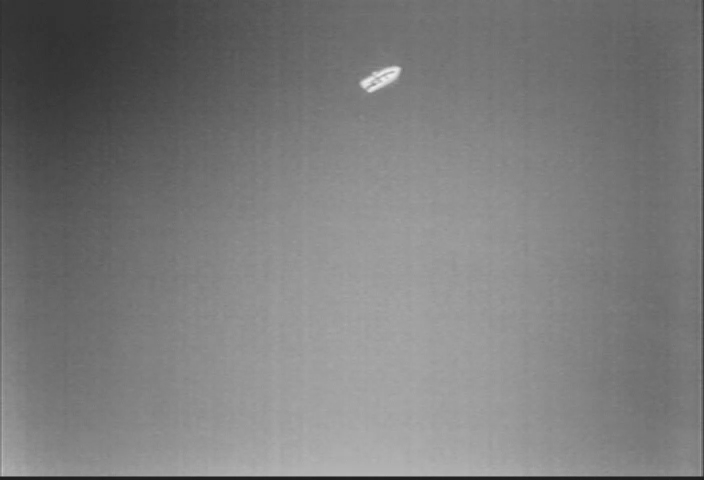
\includegraphics[width=\textwidth]{fig1}
% 		\caption{caption..}
% 		\label{fig:2a}
% 	\end{subfigure}
% 	~ %add desired spacing between images, e. g. ~, \quad, \qquad, \hfill etc.
% 	%(or a blank line to force the subfigure onto a new line)
% 	\begin{subfigure}[b]{0.45\textwidth}
% 		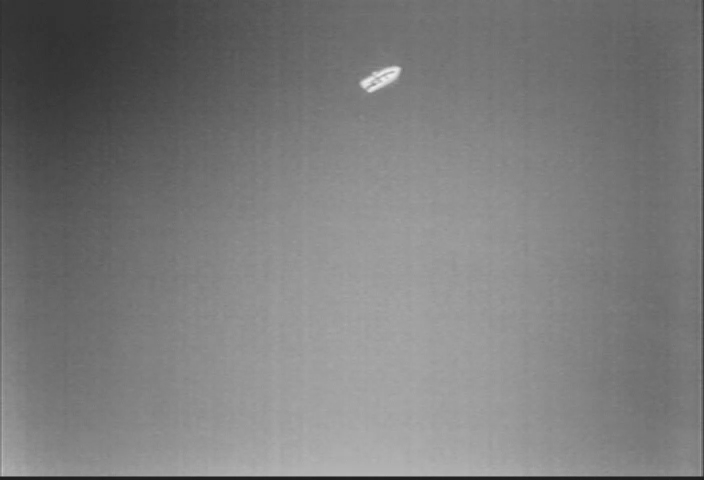
\includegraphics[width=\textwidth]{fig1}
% 		\caption{caption..}
% 		\label{fig:2b}
% 	\end{subfigure}
% 	\begin{subfigure}[b]{0.45\textwidth}
% 		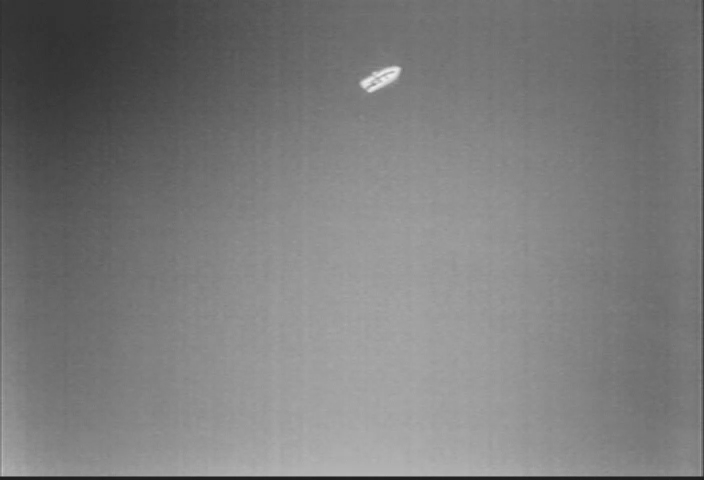
\includegraphics[width=\textwidth]{fig1}
% 		\caption{caption..}
% 		\label{fig:2c}
% 	\end{subfigure}
% 	\begin{subfigure}[b]{0.45\textwidth}
% 		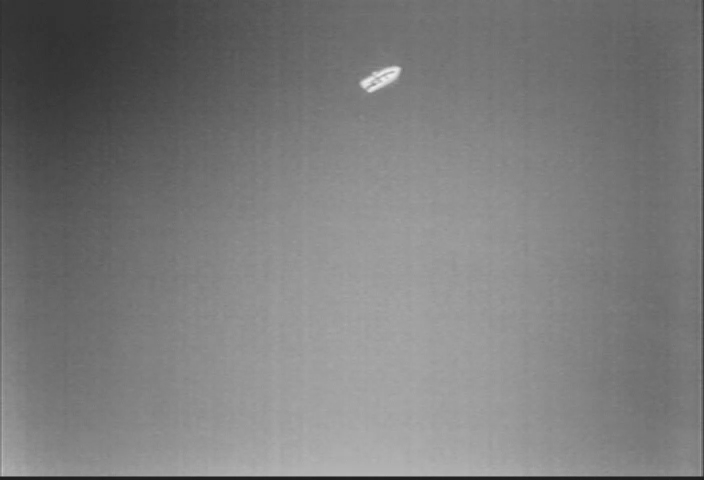
\includegraphics[width=\textwidth]{fig1}
% 		\caption{caption..}
% 		\label{fig:2d}
% 	\end{subfigure}
% 	\caption{Caption for all figures}\label{fig:2}
% \end{figure}
